\vspace{-0.25cm}

\section{Results} \label{sec:results}   
    \begin{table}
        \vspace{-0.5cm}
        
        \centering
        
        \captionsetup{singlelinecheck=false, justification=centering}
        \caption{
            \tiny
            A comparison of \gls{MAE}, \gls{RAE}, the concordance index, and the Brier score. The average survival time was approximately $32$ months. Here C refers to Classical Likelihood, EC Likelihood refers to Event Conditional Likelihood, and CF refers to when the clinical features were included in the model.
        }
        
        \vspace{-0.25cm}
        
        \resizebox*{1.0\linewidth}{0.1\textheight}
        % \resizebox*{1.0\linewidth}{!}
        {
            \begin{tabular}{||c|cc|c|c||}
                \hline
                                            & \textbf{\gls{MAE}} & \textbf{\gls{RAE}} & \textbf{C-Index}  & \textbf{Brier}    \\
                \hline
                \textbf{EC Likelihood}      & $22.7\pm1.51$      & $1.72\pm0.89$      & $0.77\pm0.05$     & $0.22\pm0.07$      \\
                \textbf{EC Likelihood CF}   & $21.5\pm1.32$      & $1.98\pm0.82$      & $0.80\pm0.03$     & $0.18\pm0.05$      \\
                \textbf{C Likelihood}       & $28.9\pm1.96$      & $2.23\pm0.01$      & $0.76\pm0.05$     & $0.25\pm0.01$      \\
                \textbf{C Likelihood CF}    & $25.3\pm1.74$      & $2.04\pm0.01$      & $0.75\pm0.04$     & $0.20\pm0.01$      \\
                \hline
                \textbf{Cox}                & $187 \pm309 $      & $17.0\pm30.7$      & $0.73\pm0.04$     & $0.61\pm0.28$      \\
                \textbf{Cox CF}             & $233 \pm287 $      & $26.4\pm21.9$      & $0.72\pm0.03$     & $0.57\pm0.16$      \\
                \textbf{Cox \gls{MB}}       & $166 \pm267 $      & $17.7\pm28.2$      & $0.74\pm0.03$     & $0.53\pm0.31$      \\
                \textbf{Cox \gls{MB} CF}    & $179 \pm294 $      & $16.3\pm22.8$      & $0.73\pm0.05$     & $0.56\pm0.24$      \\
                \hline
                \textbf{DeepHit}            & $38.4\pm14.8$      & $3.99\pm0.34$      & $0.72\pm0.03$     & $0.40\pm0.01$      \\
                \textbf{DeepHit CF}         & $31.3\pm9.19$      & $3.50\pm0.42$      & $0.71\pm0.04$     & $0.42\pm0.01$      \\
                \hline
            \end{tabular}
        }
        \label{tab:table}
        
        % \vspace{-0.5cm}
    \end{table}

    \begin{figure}
        % \vspace{-0.5cm}
        
        \centering

        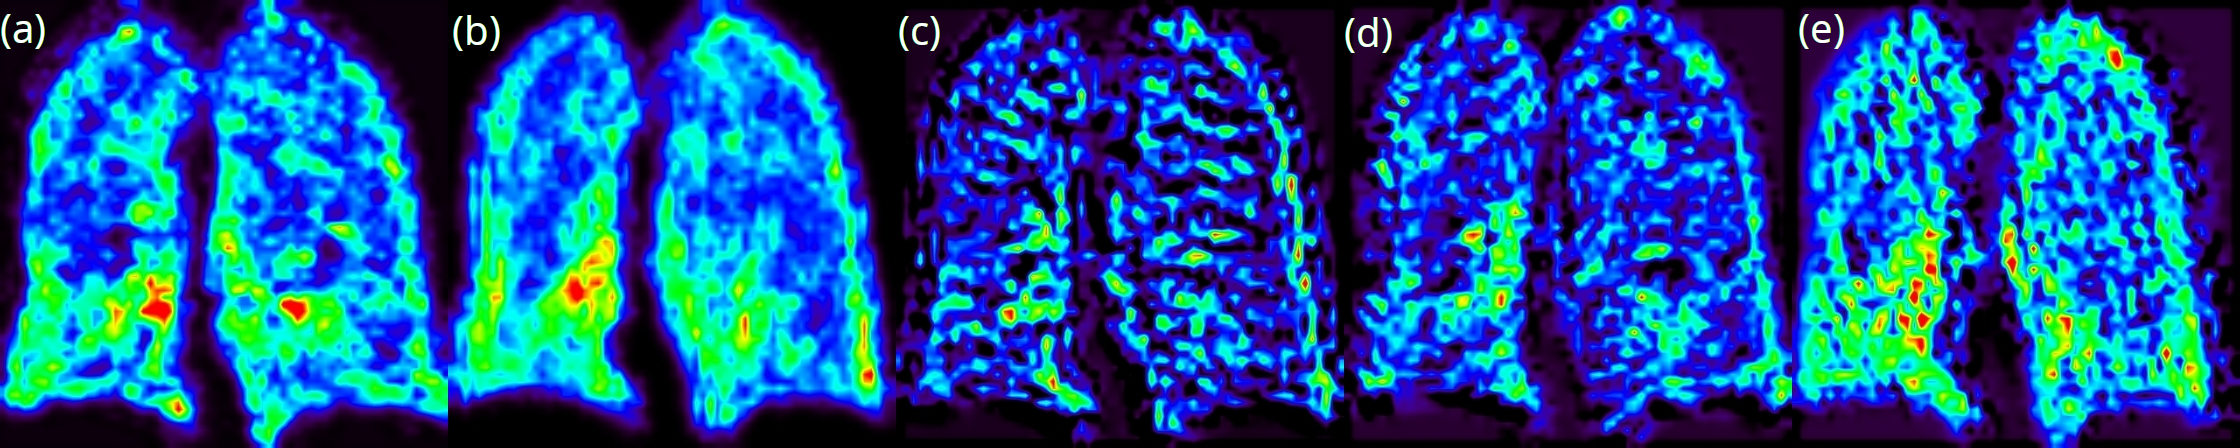
\includegraphics[width=1.0\linewidth]{Figures/grad_cam_label.png}
        % 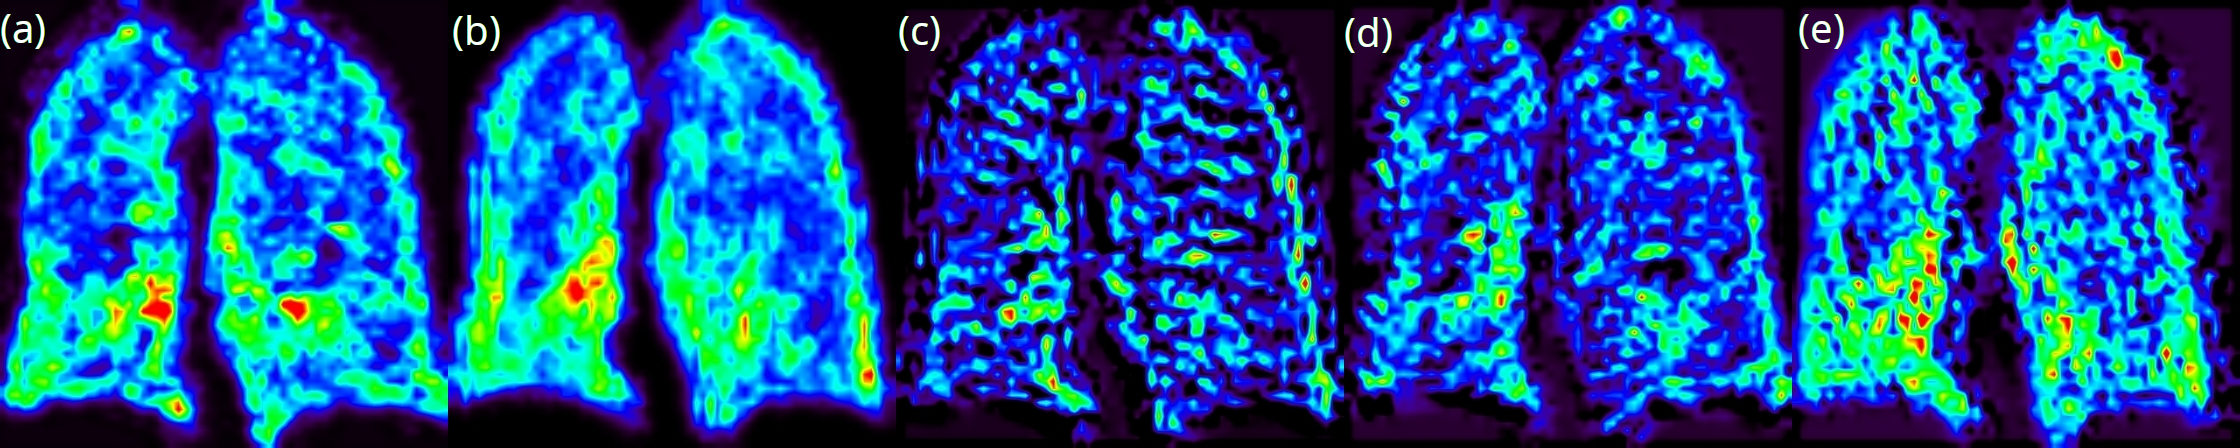
\includegraphics[width=1.0\linewidth]{Figures/grad_cam_label.png}
        
        \vspace{-0.25cm}
        
        \captionsetup{singlelinecheck=false, justification=centering}
        \caption{
            \scriptsize
            From left to right a slice through a fibrotic region of a Grad-CAM image, taken from a middle convolution, of a $65$ year old patient with a survival time of $30$ months For; (a) Death Conditional Likelihood, (b) Classical Likelihood, (c) Cox, (d) Cox \gls{MB}, and (e) DeepHit. All colour maps are consistent for all images.
        }
        \label{fig:grad_cam}
        
       \vspace{-0.5cm}
   \end{figure}

    From~\Fref{tab:table} it can be seen that the the \gls{MAE} and \gls{RAE} are often lower for both likelihood based models than for all other models. The \gls{MAE} and \gls{RAE} for the DeepHit model is lower than that of the Cox based model, while for the Cox based models not only are their errors high but they also have a substantially higher variance. The \gls{MAE} and \gls{RAE} of the Event Conditional Likelihood model is often lower than that of the Classical Likelihood model. The Brier score results also back up this assertion, however it is difficult to draw conclusions from the concordance index results. The results also seem to indicate that there is some benefit to including the clinical features, although from these results alone it is not possible to say if this is due to the added information from the clinical features or the increase in model size. From~\Fref{fig:grad_cam} it can be seen that both likelihood based model and DeepHit produced updates which identified the fibrosis in both lungs, the Cox based model only seemed to detect fibrosis in the left lung. Both likelihood models seemed to extract updates which are less noisy than the DeepHit update.
